\chapter{Comparison of Update Performance Based on Gaussian Fusion Experiments}
\label{ch:gaussian_fusion}

To objectively evaluate the discrepancy between the outputs of the filters in the update step and the corresponding analytical solutions, this chapter designs a series of single-step Gaussian fusion experiments.

According to Bayes' theorem, when both the prior distribution and the likelihood are Gaussian, their fusion yields a posterior distribution with a closed-form analytical solution, which is also Gaussian. Suppose that the prior distribution of the state vector $\vx$ is $p(\vx) = \Gaussian(\vx \mid \vmu_p, \boldsymbol{\Sigma}_p)$, and that the likelihood can be written as a Gaussian with respect to $\vx$, i.e., $p(\vy|\vx) \propto \Gaussian(\vx \mid \vmu_L, \boldsymbol{\Sigma}_L)$. After multiplication and normalization, the resulting posterior is $p(\vx|\vy) = \Gaussian(\vx \mid \vmu_e, \boldsymbol{\Sigma}_e)$. Its posterior covariance and posterior mean satisfy \cite[Section~8.1.8]{MC}
\begin{equation}
	\boldsymbol{\Sigma}_e^{-1} = \boldsymbol{\Sigma}_p^{-1} + \boldsymbol{\Sigma}_L^{-1} \enspace ,
\end{equation}
and
\begin{equation}
	\vmu_e = \boldsymbol{\Sigma}_e \left( \boldsymbol{\Sigma}_p^{-1} \vmu_p + \boldsymbol{\Sigma}_L^{-1} \vmu_L \right) \enspace .
\end{equation}

All experiments in this chapter are conducted in a 10-dimensional state space. The prior distribution is fixed as a 10D standard normal distribution. Different likelihood distributions are then introduced by varying their parameters, such as the mean and variance, to represent sensor scenarios with different noise levels and mean shifts.

The prior particles for both NFF and GPF are generated by deterministic sampling from the 10D standard normal prior. In contrast, the prior particles for PF are generated by random sampling. After constructing the prior particle sets and the likelihood functions, the update steps of the three filters are executed separately. Different particle counts are used for the three filters. Specifically, NFF uses 200, 500, 1000, and 2000 particles; GPF uses 2000, 5000, and 10000 particles; and PF uses 10000, 30000, 50000, 100000, and 300000 particles.

After the update step, the experiment computes the particle mean $\hat{\vx} = \sum_{i=1}^L w^{(i)} \vx^{(i)}$ and covariance $\mP = \sum_{i=1}^L w^{(i)} (\vx^{(i)} - \hat{\vx})(\vx^{(i)} - \hat{\vx})^{\top}$. These quantities are then compared with the analytical posterior mean and covariance given above. Finally, the RMSE between the filtered mean and the analytical posterior mean, as well as the RFE between the estimated particle covariance and the analytical posterior covariance, are evaluated.
\section{Likelihood Variance Sensitivity Analysis}
\label{sec:likelihood_sensitivity}

This set of experiments investigates how the variance of the observation likelihood affects the accuracy of different filters. In this experiment, the likelihood mean is fixed at $\vmu_L = \vones$ for all dimensions, i.e., the mean shift is 1 in every dimension, and the likelihood covariance matrix is set to $\boldsymbol{\Sigma}_L = \sigma_L^2 \mI_{10}$. The control variable is the likelihood variance, with $\sigma_L^2$ varying from 0.1 to 10.

The RMSE and RFE of each filter under different likelihood variances are shown in \Fig{fig:likelihood_variance_results}.

\begin{Figure}[ht]
	\centering
	% Row 1: L=200
	\begin{SubFigure}{0.48\textwidth}
		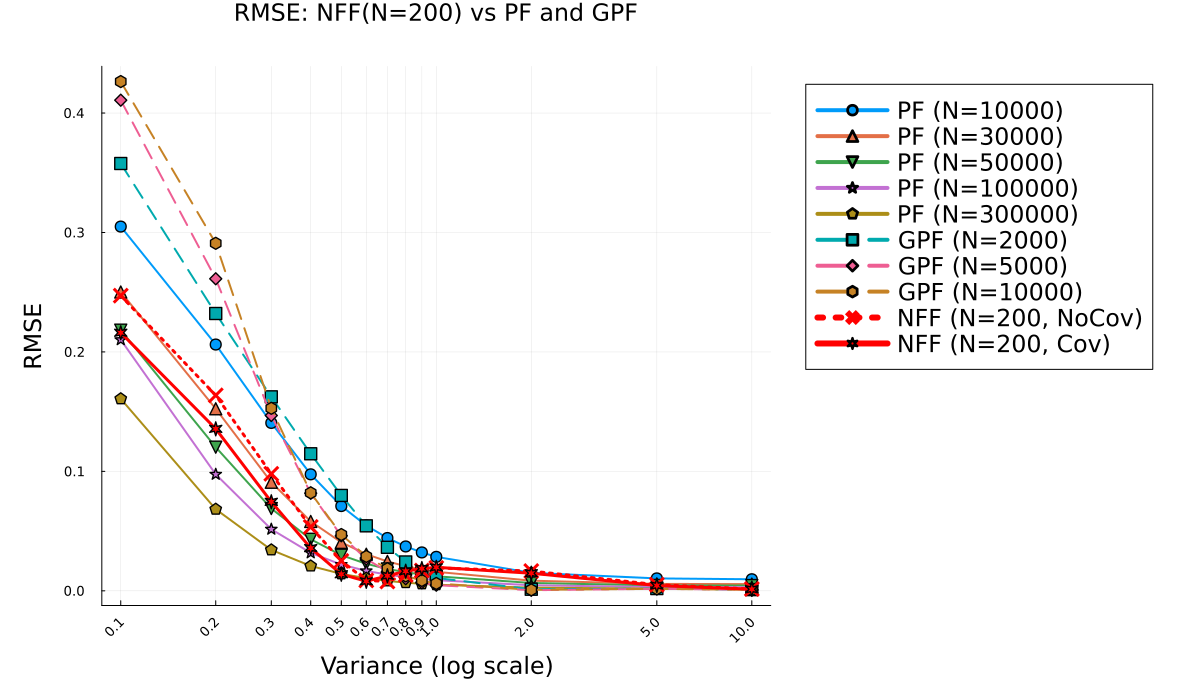
\includegraphics[width=\textwidth]{figures/Experiment01/rmse_NFF_CG_N200_vs_others.png}
		\caption{RMSE, $L=200$}
	\end{SubFigure}
	\hfill
	\begin{SubFigure}{0.48\textwidth}
		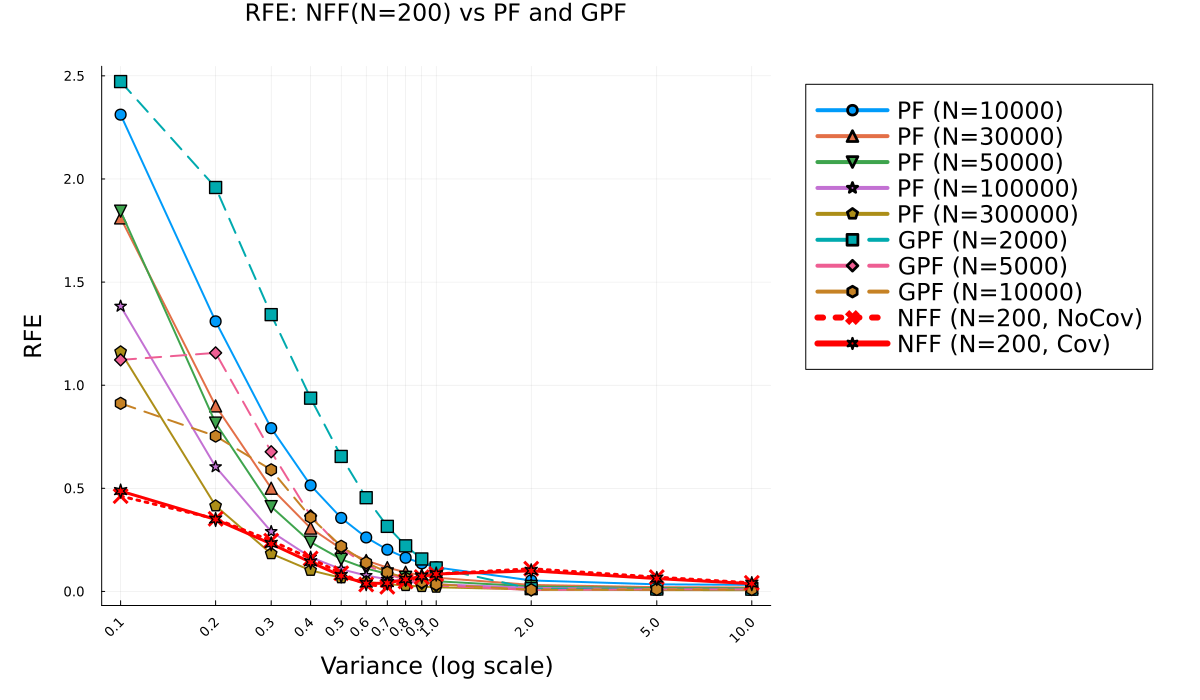
\includegraphics[width=\textwidth]{figures/Experiment01/rel_frob_NFF_CG_N200_vs_others.png}
		\caption{RFE, $L=200$}
	\end{SubFigure}
	
	\vspace{1em}
	
	% Row 2: L=500
	\begin{SubFigure}{0.48\textwidth}
		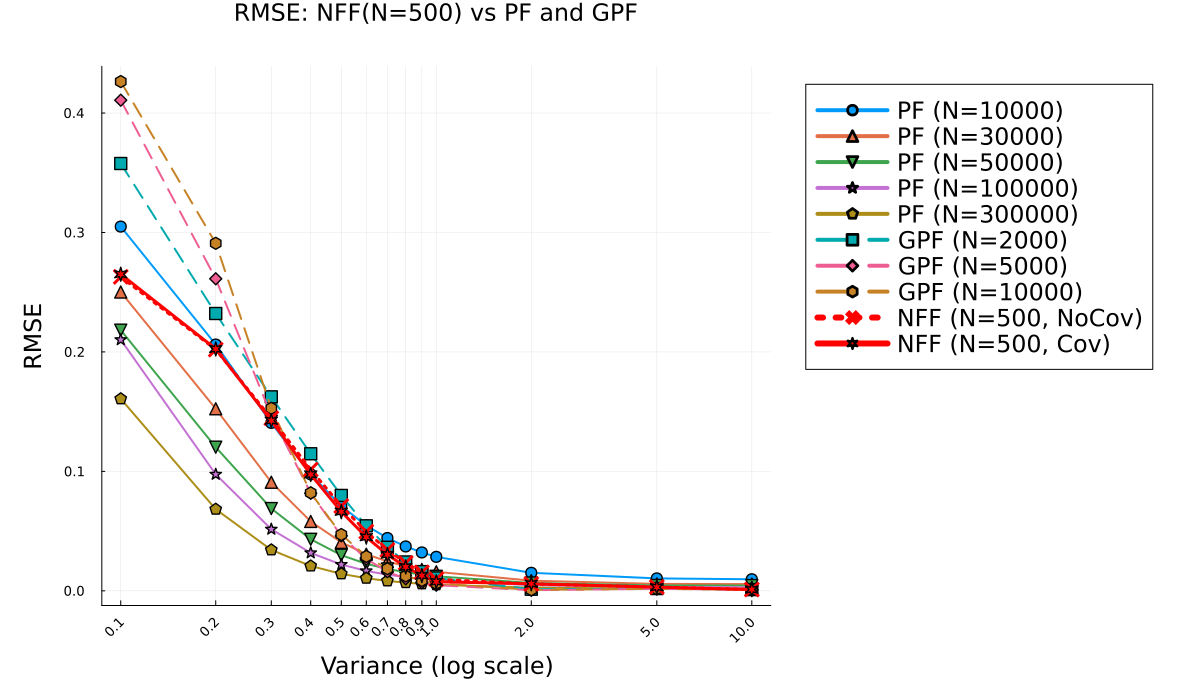
\includegraphics[width=\textwidth]{figures/Experiment01/rmse_NFF_CG_N500_vs_others.png}
		\caption{RMSE, $L=500$}
	\end{SubFigure}
	\hfill
	\begin{SubFigure}{0.48\textwidth}
		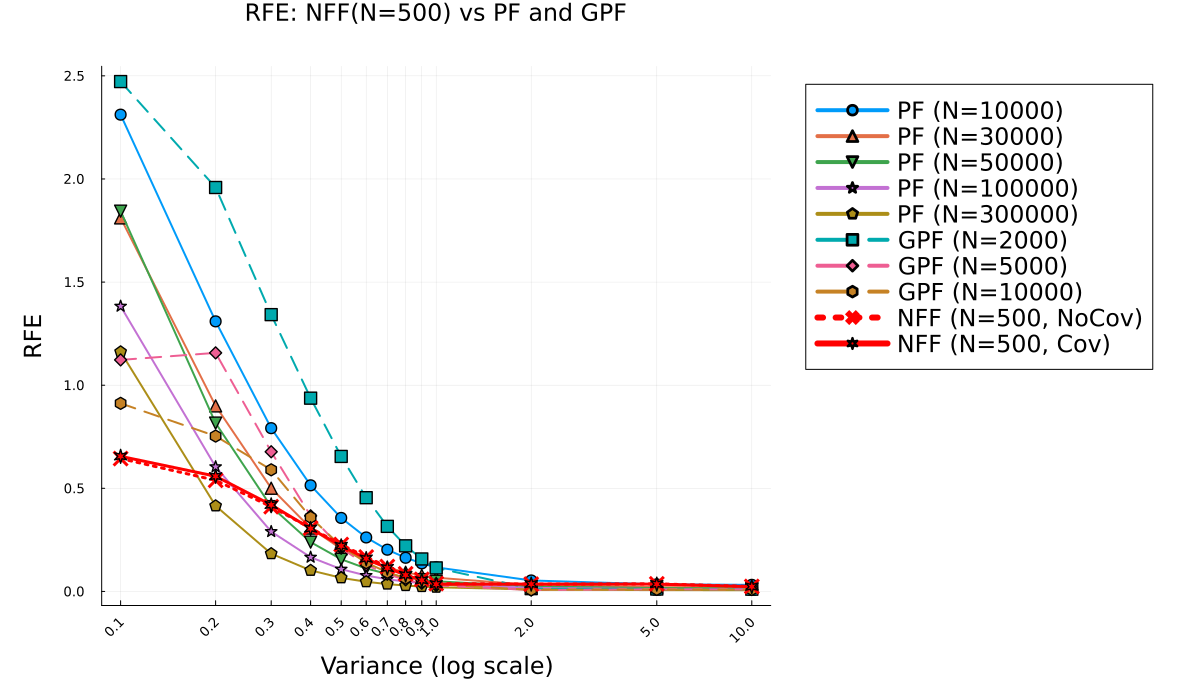
\includegraphics[width=\textwidth]{figures/Experiment01/rel_frob_NFF_CG_N500_vs_others.png}
		\caption{RFE, $L=500$}
	\end{SubFigure}
	
	\vspace{1em}
	
	% Row 3: L=1000
	\begin{SubFigure}{0.48\textwidth}
		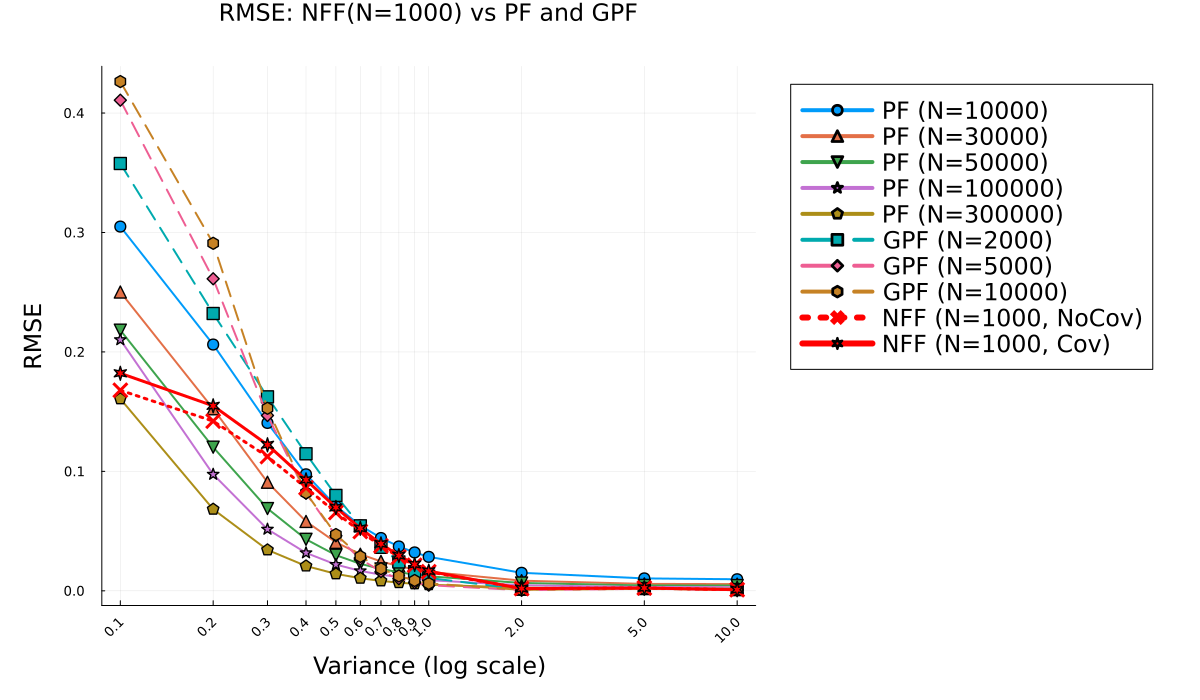
\includegraphics[width=\textwidth]{figures/Experiment01/rmse_NFF_CG_N1000_vs_others.png}
		\caption{RMSE, $L=1000$}
	\end{SubFigure}
	\hfill
	\begin{SubFigure}{0.48\textwidth}
		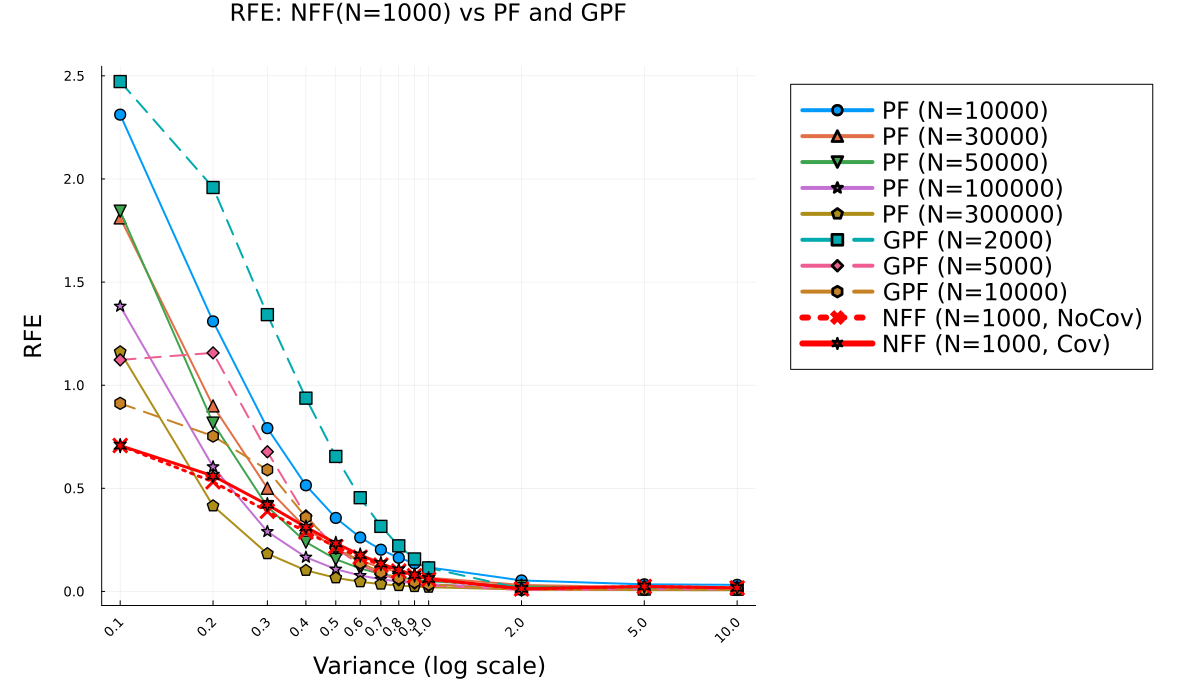
\includegraphics[width=\textwidth]{figures/Experiment01/rel_frob_NFF_CG_N1000_vs_others.png}
		\caption{RFE, $L=1000$}
	\end{SubFigure}
	
	\vspace{1em}
	
	% Row 4: L=2000
	\begin{SubFigure}{0.48\textwidth}
		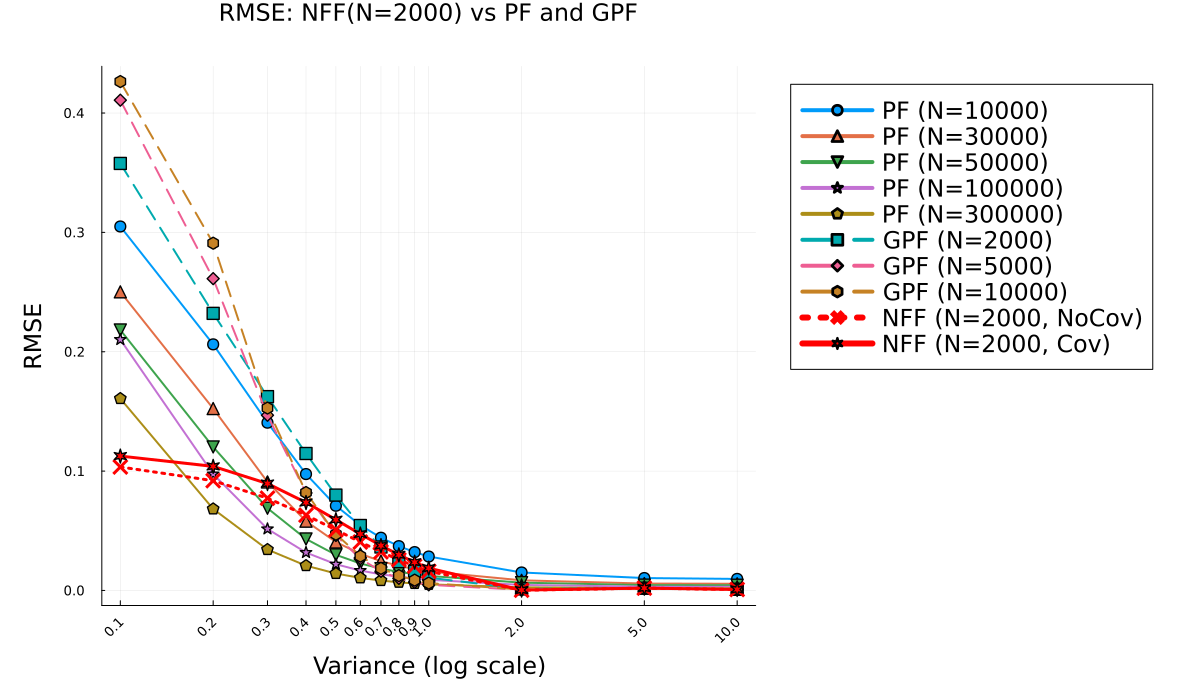
\includegraphics[width=\textwidth]{figures/Experiment01/rmse_NFF_CG_N2000_vs_others.png}
		\caption{RMSE, $L=2000$}
	\end{SubFigure}
	\hfill
	\begin{SubFigure}{0.48\textwidth}
		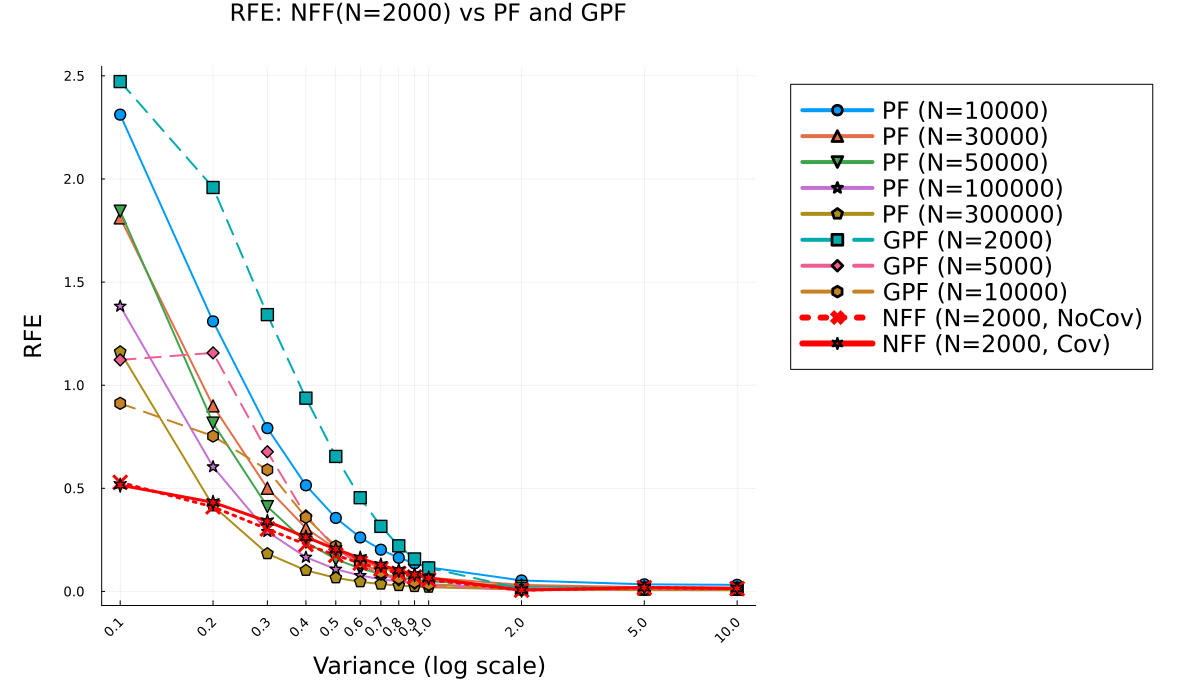
\includegraphics[width=\textwidth]{figures/Experiment01/rel_frob_NFF_CG_N2000_vs_others.png}
		\caption{RFE, $L=2000$}
	\end{SubFigure}
	
	\caption{RMSE and RFE vs. $\sigma_L^2$}
	\label{fig:likelihood_variance_results}
\end{Figure}

From \Fig{fig:likelihood_variance_results}, the following main conclusions can be drawn:

Regardless of the filtering algorithm, as the likelihood variance $\sigma_L^2$ decreases, both the mean estimation error and the covariance estimation error increase for all filters.

When the likelihood variance becomes very small, the covariance estimation errors of PF and GPF deteriorate rapidly. In contrast, the increase in the covariance estimation error of NFF is noticeably more gradual. In the likelihood variance range of $0.3 \sim 1.0$, the covariance estimation accuracy of NFF is comparable to that of PF with 50000 particles and GPF with 10000 particles. In the range $0.2 \sim 0.3$, NFF performs comparably to PF with 100000 to 300000 particles. When the likelihood variance becomes extremely small, in the range $0.1 \sim 0.2$, the covariance estimation accuracy of NFF even surpasses that of PF with 300000 particles.

With a relatively small number of particles (e.g., $L=200, 500$), the mean estimation accuracy of NFF, measured by RMSE, is comparable to that of PF with 10000 to 50000 particles. With a larger number of particles (e.g., $L=1000, 2000$), under extremely narrow likelihoods ($0.1 \sim 0.2$), the mean estimation accuracy of NFF also exceeds that of PF with 300000 particles. This indicates that the smaller the likelihood variance, the more pronounced the advantage of NFF becomes.

\subsection*{Why does a narrow likelihood lead to worse estimation results?}

For PF and GPF, the main cause of the error increase is severe particle degeneracy. When the likelihood variance is very small, the likelihood becomes sharply concentrated. In this case, most prior particles lie outside the effective support of the likelihood. During the update step, almost all particle weights approach zero. As a result, the number of effective particles drops sharply, and the filter loses its ability to approximate the posterior distribution.

For NFF, the error mainly arises from the sparsity of high-dimensional space and the information loss introduced during the approximation process. As the ODE drives the particles from the prior toward the posterior, the true posterior density is continuously approximated by an equal-weight particle representation. This process inevitably introduces information loss. Moreover, in a 10D state space, even 2000 particles remain highly sparse. When the likelihood is extremely sharp, its peak can easily fall into the large gaps between particles, which leads to additional information loss and less accurate estimates.

\subsection*{Why does a narrower likelihood increase the computation time of NFF?}

\begin{Figure}[ht]
	\centering
	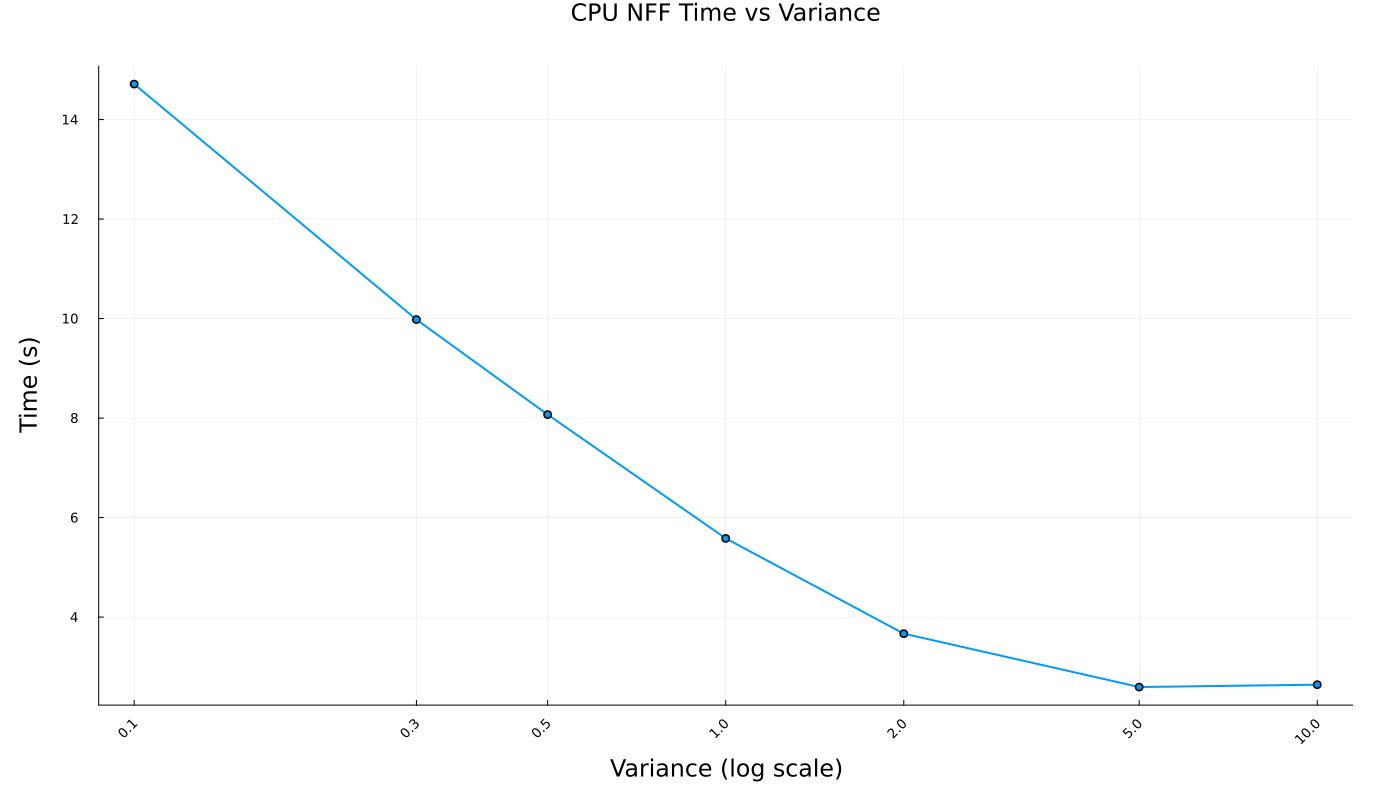
\includegraphics[width=0.9\textwidth]{figures/Experiment01/cpu_benchmark.png}
	\caption{CPU time vs. $\sigma_L^2$.}
	\label{fig:cpu_benchmark01}
\end{Figure}

As shown in \Fig{fig:cpu_benchmark01}, the single-step update time of NFF increases sharply as the likelihood variance decreases. As discussed in \SubSec{subsec:vcabm}, a narrower likelihood results in a stiffer ODE, which forces the VCABM integrator to take significantly more time to solve it.

\clearpage

\section{Prior-Likelihood Distance Sensitivity Analysis}
\label{sec:prior_likelihood_distance}

This experiment investigates the effect of the distance between the prior mean and the likelihood mean on the update accuracy of different filters. In this experiment, the likelihood covariance matrix is fixed at $\boldsymbol{\Sigma}_L = \mI_{10}$.

The control variable is the mean shift of the likelihood, with the likelihood mean $\vmu_L$ gradually increasing from 0.1 to 10.0. As this mean shift increases, the physical distance between the sensor observation region and the system prediction region also increases.

The RMSE and RFE of the filters under different mean shifts are shown in \Fig{fig:mean_shift_results}.

\begin{Figure}[ht]
	\centering
	% Row 1: L=200
	\begin{SubFigure}{0.48\textwidth}
		
\includegraphics[width=\textwidth]{figures/Experiment02/rmse_NFF_CG_N200_vs_others.png}
		\caption{RMSE, $L=200$}
		\label{fig:mean_shift_rmse_200}
	\end{SubFigure}
	\hfill
	\begin{SubFigure}{0.48\textwidth}
		
\includegraphics[width=\textwidth]{figures/Experiment02/rel_frob_NFF_CG_N200_vs_others.png}
		\caption{Rel. Frobenius Error, $L=200$}
		\label{fig:mean_shift_frob_200}
	\end{SubFigure}
	
	\vspace{1em}
	
	% Row 2: L=500
	\begin{SubFigure}{0.48\textwidth}
		
\includegraphics[width=\textwidth]{figures/Experiment02/rmse_NFF_CG_N500_vs_others.png}
		\caption{RMSE, $L=500$}
		\label{fig:mean_shift_rmse_500}
	\end{SubFigure}
	\hfill
	\begin{SubFigure}{0.48\textwidth}
		
\includegraphics[width=\textwidth]{figures/Experiment02/rel_frob_NFF_CG_N500_vs_others.png}
		\caption{Rel. Frobenius Error, $L=500$}
		\label{fig:mean_shift_frob_500}
	\end{SubFigure}
	
	\vspace{1em}
	
	% Row 3: L=1000
	\begin{SubFigure}{0.48\textwidth}
		
\includegraphics[width=\textwidth]{figures/Experiment02/rmse_NFF_CG_N1000_vs_others.png}
		\caption{RMSE, $L=1000$}
		\label{fig:mean_shift_rmse_1000}
	\end{SubFigure}
	\hfill
	\begin{SubFigure}{0.48\textwidth}
		
\includegraphics[width=\textwidth]{figures/Experiment02/rel_frob_NFF_CG_N1000_vs_others.png}
		\caption{Rel. Frobenius Error, $L=1000$}
		\label{fig:mean_shift_frob_1000}
	\end{SubFigure}
	
	\vspace{1em}
	
	% Row 4: L=2000
	\begin{SubFigure}{0.48\textwidth}
		
\includegraphics[width=\textwidth]{figures/Experiment02/rmse_NFF_CG_N2000_vs_others.png}
		\caption{RMSE, $L=2000$}
		\label{fig:mean_shift_rmse_2000}
	\end{SubFigure}
	\hfill
	\begin{SubFigure}{0.48\textwidth}
		
\includegraphics[width=\textwidth]{figures/Experiment02/rel_frob_NFF_CG_N2000_vs_others.png}
		\caption{Rel. Frobenius Error, $L=2000$}
		\label{fig:mean_shift_frob_2000}
	\end{SubFigure}
	
	\caption{RMSE and RFE vs. likelihood mean.}
	\label{fig:mean_shift_results}
\end{Figure}

From \Fig{fig:mean_shift_results}, the following main conclusions can be drawn:

As the likelihood distribution moves farther away from the prior distribution, both the mean estimation error and the covariance estimation error increase across all filtering algorithms.

When the likelihood mean shift lies in the large-deviation range from 1.5 to 10.0, the RMSE and RFE of PF and GPF increase dramatically, and these filters effectively fail. In contrast, the error of NFF remains at a very low level. This indicates that the farther the likelihood is from the prior, the more pronounced the advantage of NFF becomes.

\subsection*{Why do more distant likelihoods lead to less accurate estimates?}

PF and GPF fail under distant likelihoods because they suffer from severe particle degeneracy.

For NFF, as discussed earlier, the particle flow continuously replaces the true posterior density by an approximate posterior density. This repeated approximation inevitably introduces information loss throughout the flow process.

\subsection*{Why does a more distant likelihood increase the computation time of NFF?}

\begin{Figure}[ht]
	\centering
	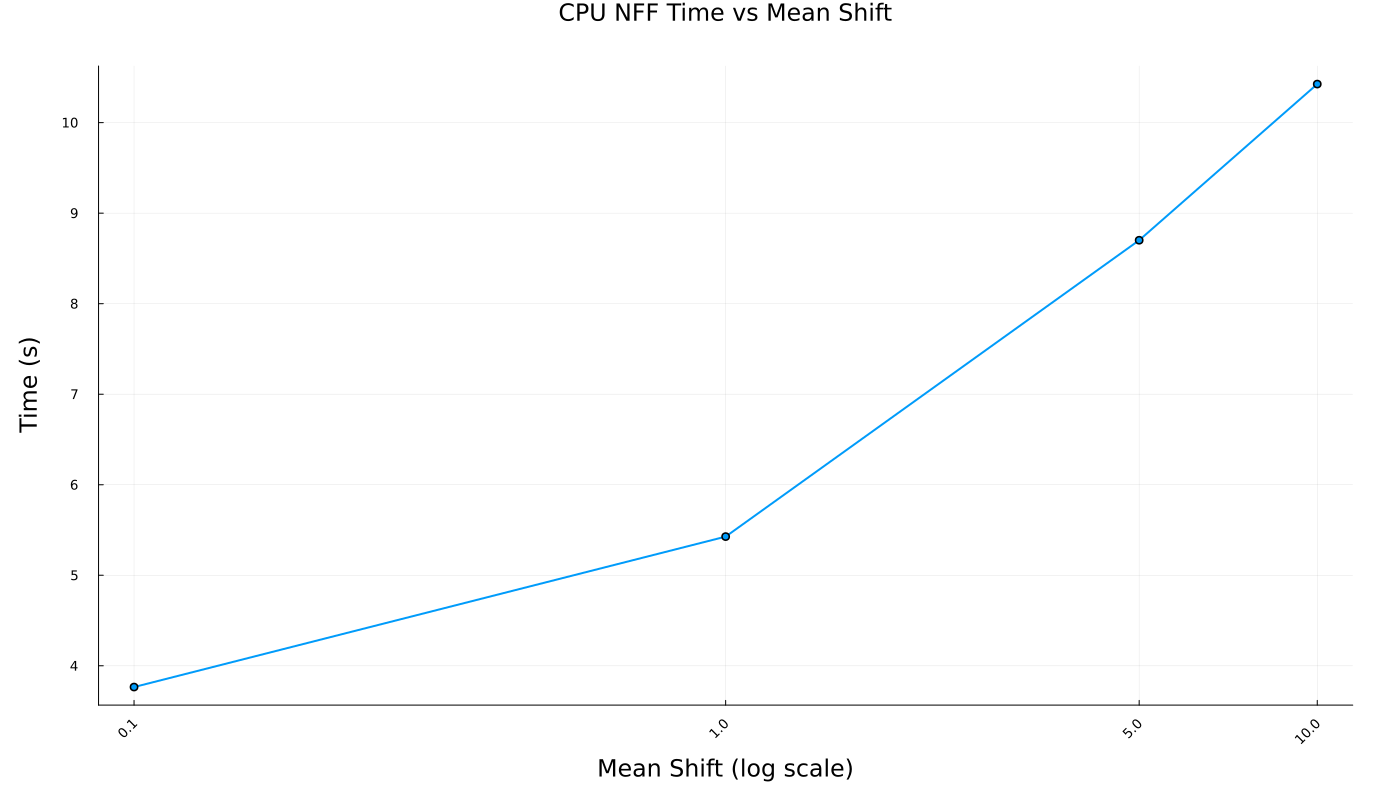
\includegraphics[width=0.9\textwidth]{figures/Experiment02/time_benchmark.png}
	\caption{CPU update time vs. likelihood mean.}
	\label{fig:cpu_benchmark02}
\end{Figure}

This correlation between the likelihood mean and the computational cost is demonstrated in \Fig{fig:cpu_benchmark02}. As discussed earlier in \SubSec{subsec:vcabm}, when the initial particle cloud is very far from the effective support of the likelihood, the ODE becomes highly stiff. As a result, the VCABM integrator must use much smaller step sizes to maintain accuracy, which significantly increases the total computation time.

\clearpage

\section{Influence of State Dimension}
\label{sec:influence_dimension}

To investigate how the state dimension affects filtering accuracy, this experiment uses the state dimension $N$ as the control variable and increases it gradually from 2 to 20.

In these experiments, the prior and likelihood parameters are fixed. The likelihood covariance is set to $\boldsymbol{\Sigma}_L = 0.3 \mI_N$, and the mean in each dimension is fixed at 5, such that $\vmu_L = [5, 5, \dots, 5]^{\top}$.

When comparing mean estimation accuracy across different dimensions, RMSE is not an appropriate metric. This is because as the dimension $N$ increases, the norm of the true posterior mean vector $\vmu_\text{true}$ also increases naturally. To remove this scaling effect, this experiment uses the Relative Mean Error (RME) as the main metric given by
\begin{equation}
	\text{RME} = \frac{||\hat{\vx} - \vmu_\text{true}||}{||\vmu_\text{true}||} \enspace .
\end{equation}
RME provides a dimensionless benchmark for comparing performance across different state dimensions.

The RME and RFE of the filters under different state dimensions are shown in \Fig{fig:dimension_results}.

\begin{Figure}[ht]
	\centering
	\begin{SubFigure}{0.48\textwidth}
		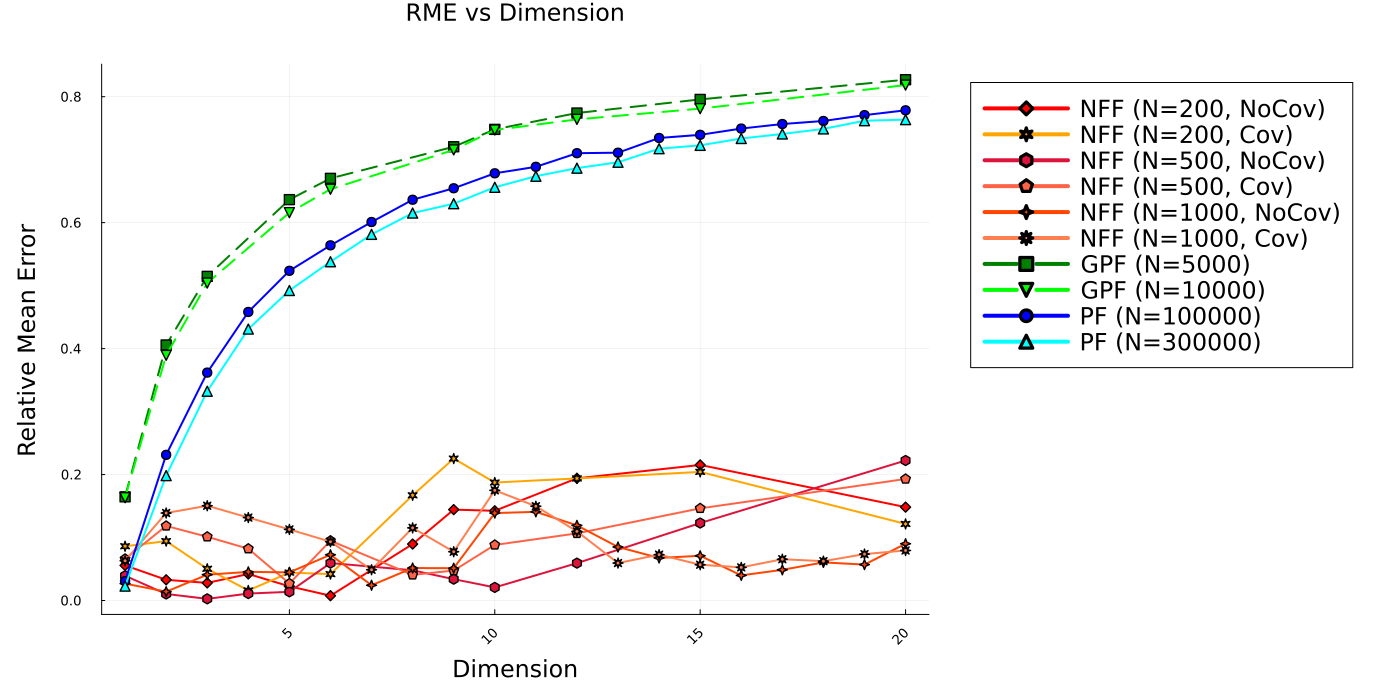
\includegraphics[width=\textwidth]{figures/Experiment04/e_mu.png}
		\caption{RME vs. Dimension.}
		\label{fig:rme_vs_dim}
	\end{SubFigure}
	\hfill
	\begin{SubFigure}{0.48\textwidth}
		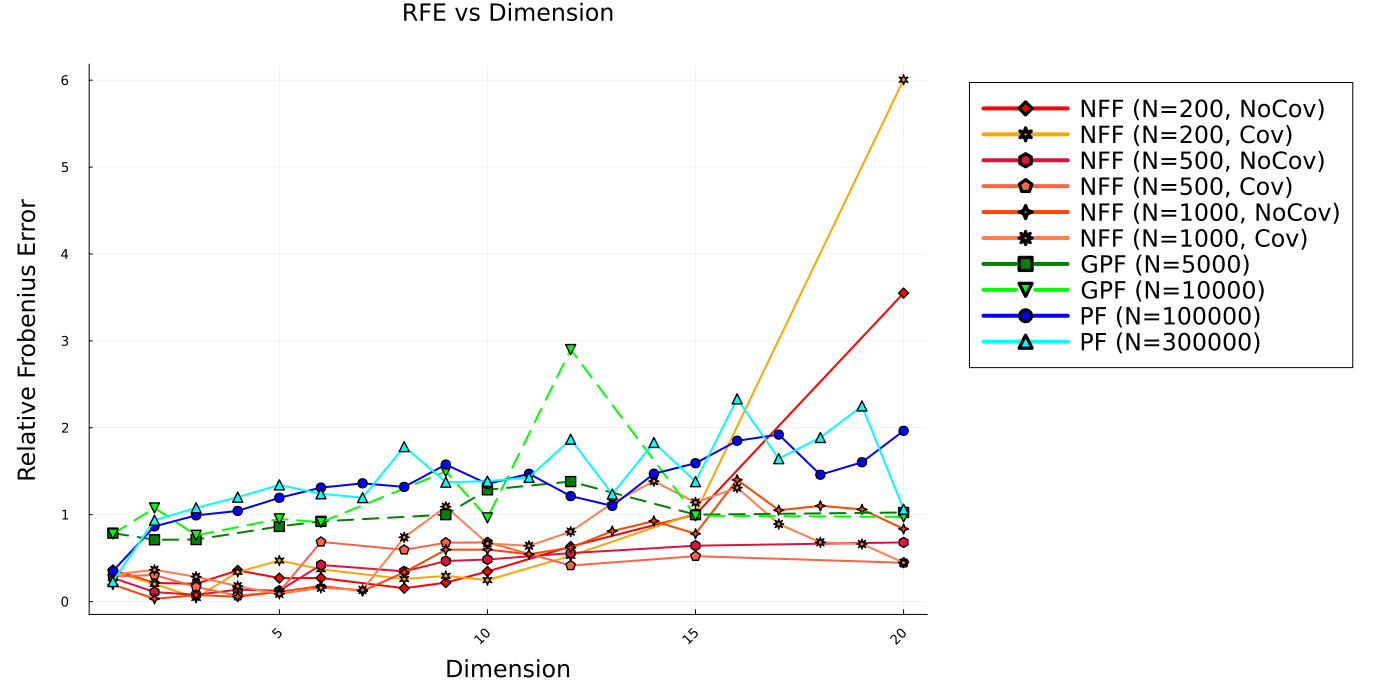
\includegraphics[width=\textwidth]{figures/Experiment04/rel_frob.png}
		\caption{RFE vs. Dimension.}
		\label{fig:frob_vs_dim}
	\end{SubFigure}
	\caption{RME and RFE vs. dimension.}
	\label{fig:dimension_results}
\end{Figure}

The following conclusions can be drawn:

Within the tested range from 2 to 20 dimensions, the mean estimation accuracy of PF and GPF deteriorates rapidly as the dimension increases. At 20 dimensions, their RME exceeds 0.8, indicating that the filters have essentially lost track of the target. In contrast, the RME of NFF changes only slightly and remains stable below 0.2.

When the state dimension satisfies $N \in [2, 15]$, the RFE of NFF remains below 1.0, and its covariance estimation accuracy is better than that of PF with 300000 particles. When the dimension increases further from 15 to 20, the relative Frobenius error of NFF with 200 or 500 particles rises sharply because of the limited particle number. However, the covariance estimation accuracy of NFF with 1000 particles is still comparable to that of GPF with 10000 particles and remains better than that of PF. Compared with PF and GPF, NFF is therefore better suited to state estimation in high-dimensional spaces.

\clearpage

\section{Parameter Analysis of NFF}
\label{sec:parameter_analysis}

This section presents a sensitivity analysis of the internal parameters of NFF under a baseline scenario in which the prior is a standard normal distribution, the likelihood mean is fixed at $\vmu_L = [5, 5, \dots, 5]^{\top}$, and the likelihood covariance is fixed at $\boldsymbol{\Sigma}_L = 0.3 \mI_{10}$.

\subsection{Influence of Particle Count}
\label{subsec:particle_count_impact}

This experiment evaluates the performance of NFF for different particle counts ($L \in [100, 2000]$) and compares the resulting errors with those of PF and GPF. The results are shown in \Fig{fig:nff_parameter_L}.

\begin{Figure}[ht]
	\centering
	\begin{SubFigure}{\textwidth}
		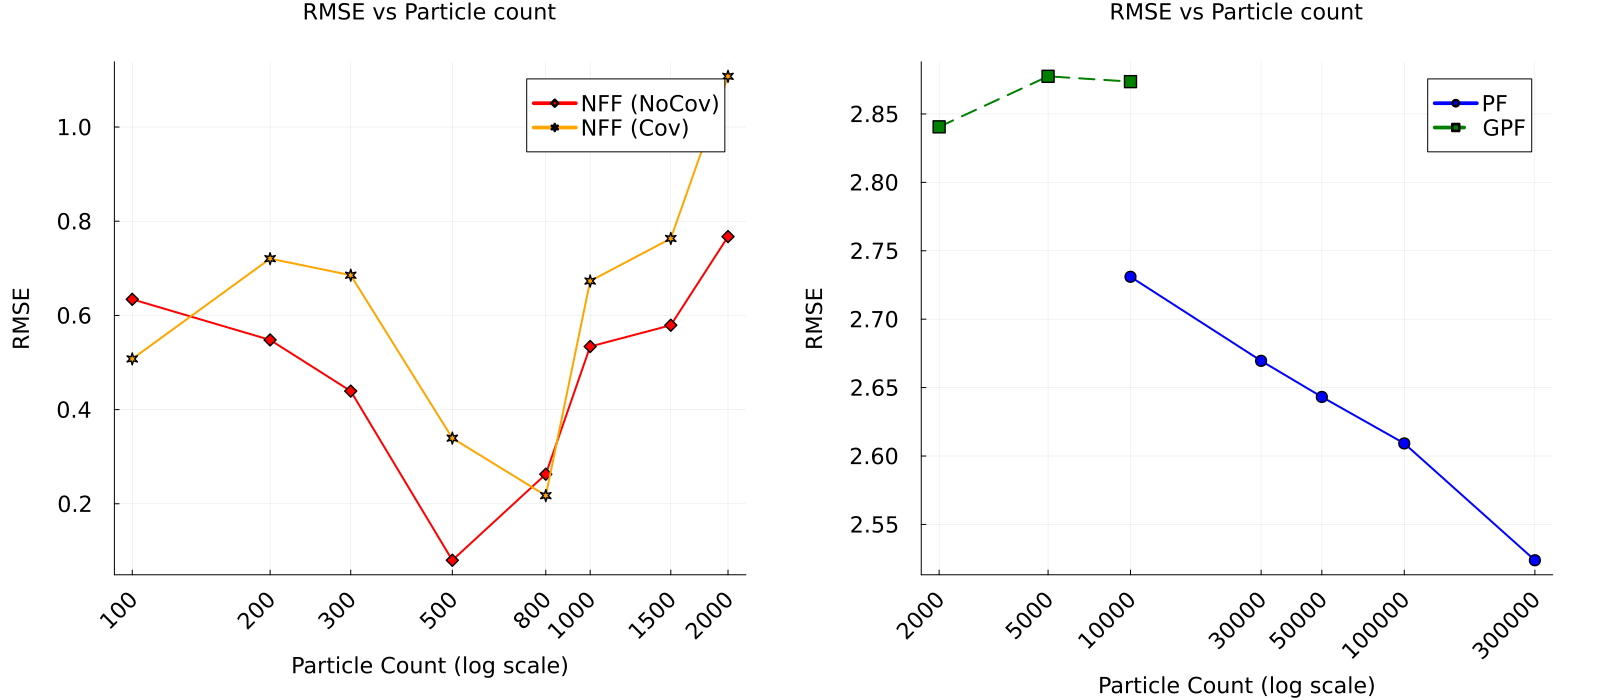
\includegraphics[width=\textwidth]{figures/Experiment3.1/rmse.png}
		\caption{RMSE vs. particle count $L$.}
		\label{fig:nff_rmse_L}
	\end{SubFigure}
	
	\vspace{1.5em}
	
	\begin{SubFigure}{\textwidth}
		
\includegraphics[width=\textwidth]{figures/Experiment3.1/rel_frob.png}
		\caption{RFE vs. particle count $L$.}
		\label{fig:nff_frob_L}
	\end{SubFigure}
	
	\caption{RMSE and RFE vs. particle count $L$}
	\label{fig:nff_parameter_L}
\end{Figure}

\textbf{U-shaped trend in mean estimation error:} As shown in the results, unlike standard particle filters, for which a larger number of particles usually improves mean estimation accuracy, the mean estimation error of NFF exhibits a U-shaped trend as the particle count increases. This indicates that, for NFF mean estimation, more particles are not always beneficial.

When the number of particles is too small (e.g., 100--200), the particle distribution is too sparse in the 10D state space to approximate the true posterior effectively, which leads to a large mean estimation error. However, when the number of particles becomes too large (e.g., 1000--2000), the cross terms in the modified Cramér--von Mises distance \Eq{eq:CVM_Dxy} become extremely numerous and complex. The increasing contribution of these cross terms weakens the relative influence of the mean-difference term ($D_E$) in the optimization objective. As a result, the algorithm must operate in a balanced particle range, such as 300--500 particles in the present scenario, which is sufficiently dense to approximate the distribution while avoiding excessive cross-term complexity.

Regarding covariance estimation, the relative Frobenius error shows that the accuracy is poor when the particle count is small. The error decreases rapidly and reaches its minimum when the particle count is around 300. Beyond this point, although the covariance error fluctuates slightly as more particles are added, it remains within a reasonable range, stays below 1.0, and performs significantly better than PF.

\textbf{Constraint comparison:} Comparing NFF with and without covariance constraints shows that, in the present scenario, the constrained version is actually less accurate in estimating both the mean and the covariance than the unconstrained version. This disadvantage is especially pronounced when the number of particles is large.

NFF with covariance constraints adds the second-moment penalty term \Eq{eq:D_Cov} to the CVM optimization objective. In order to reduce the discrepancy in the second moment, the algorithm must compromise on the optimization of the first moment and the higher-order distribution structure represented by the kernel cross terms. This multi-objective trade-off leads to a reduction in overall estimation accuracy when covariance constraints are imposed.
\clearpage

\subsection{Selection of the Homotopy Function}
\label{subsec:homotopy_function_selection}

In NFF, the homotopy function must satisfy the boundary conditions $g(0)=0$ and $g(1)=1$, but its path within the interval $\gamma \in (0, 1)$ can be chosen freely. To investigate how the shape of the homotopy function affects filtering accuracy and computational efficiency, this section compares five different homotopy functions and their corresponding derivatives $\dot{g}(\gamma)$.

The tested functions include a linear function $g(\gamma) = \gamma$ with derivative $\dot{g}(\gamma) = 1.0$, and a convex function $g(\gamma) = \gamma^2$ with derivative $\dot{g}(\gamma) = 2\gamma$. In addition, a concave function $g(\gamma) = -\gamma^2 + 2\gamma$ with derivative $\dot{g}(\gamma) = -2\gamma + 2$ is evaluated. More complex paths are also considered, including a convex-then-concave function
$g(\gamma) = \frac{1}{2}\sin(\pi\gamma - \frac{\pi}{2}) + \frac{1}{2}$
with derivative
$\dot{g}(\gamma) = \frac{\pi}{2}\cos(\pi\gamma - \frac{\pi}{2})$,
and a concave-then-convex function
$g(\gamma) = \gamma^3 - \frac{3}{2}\gamma^2 + \frac{3}{2}\gamma$
with derivative
$\dot{g}(\gamma) = 3\gamma^2 - 3\gamma + 1.5$. These homotopy functions and their corresponding derivatives are illustrated in \Fig{fig:function_plots}.

\begin{Figure}[ht]
    \centering
    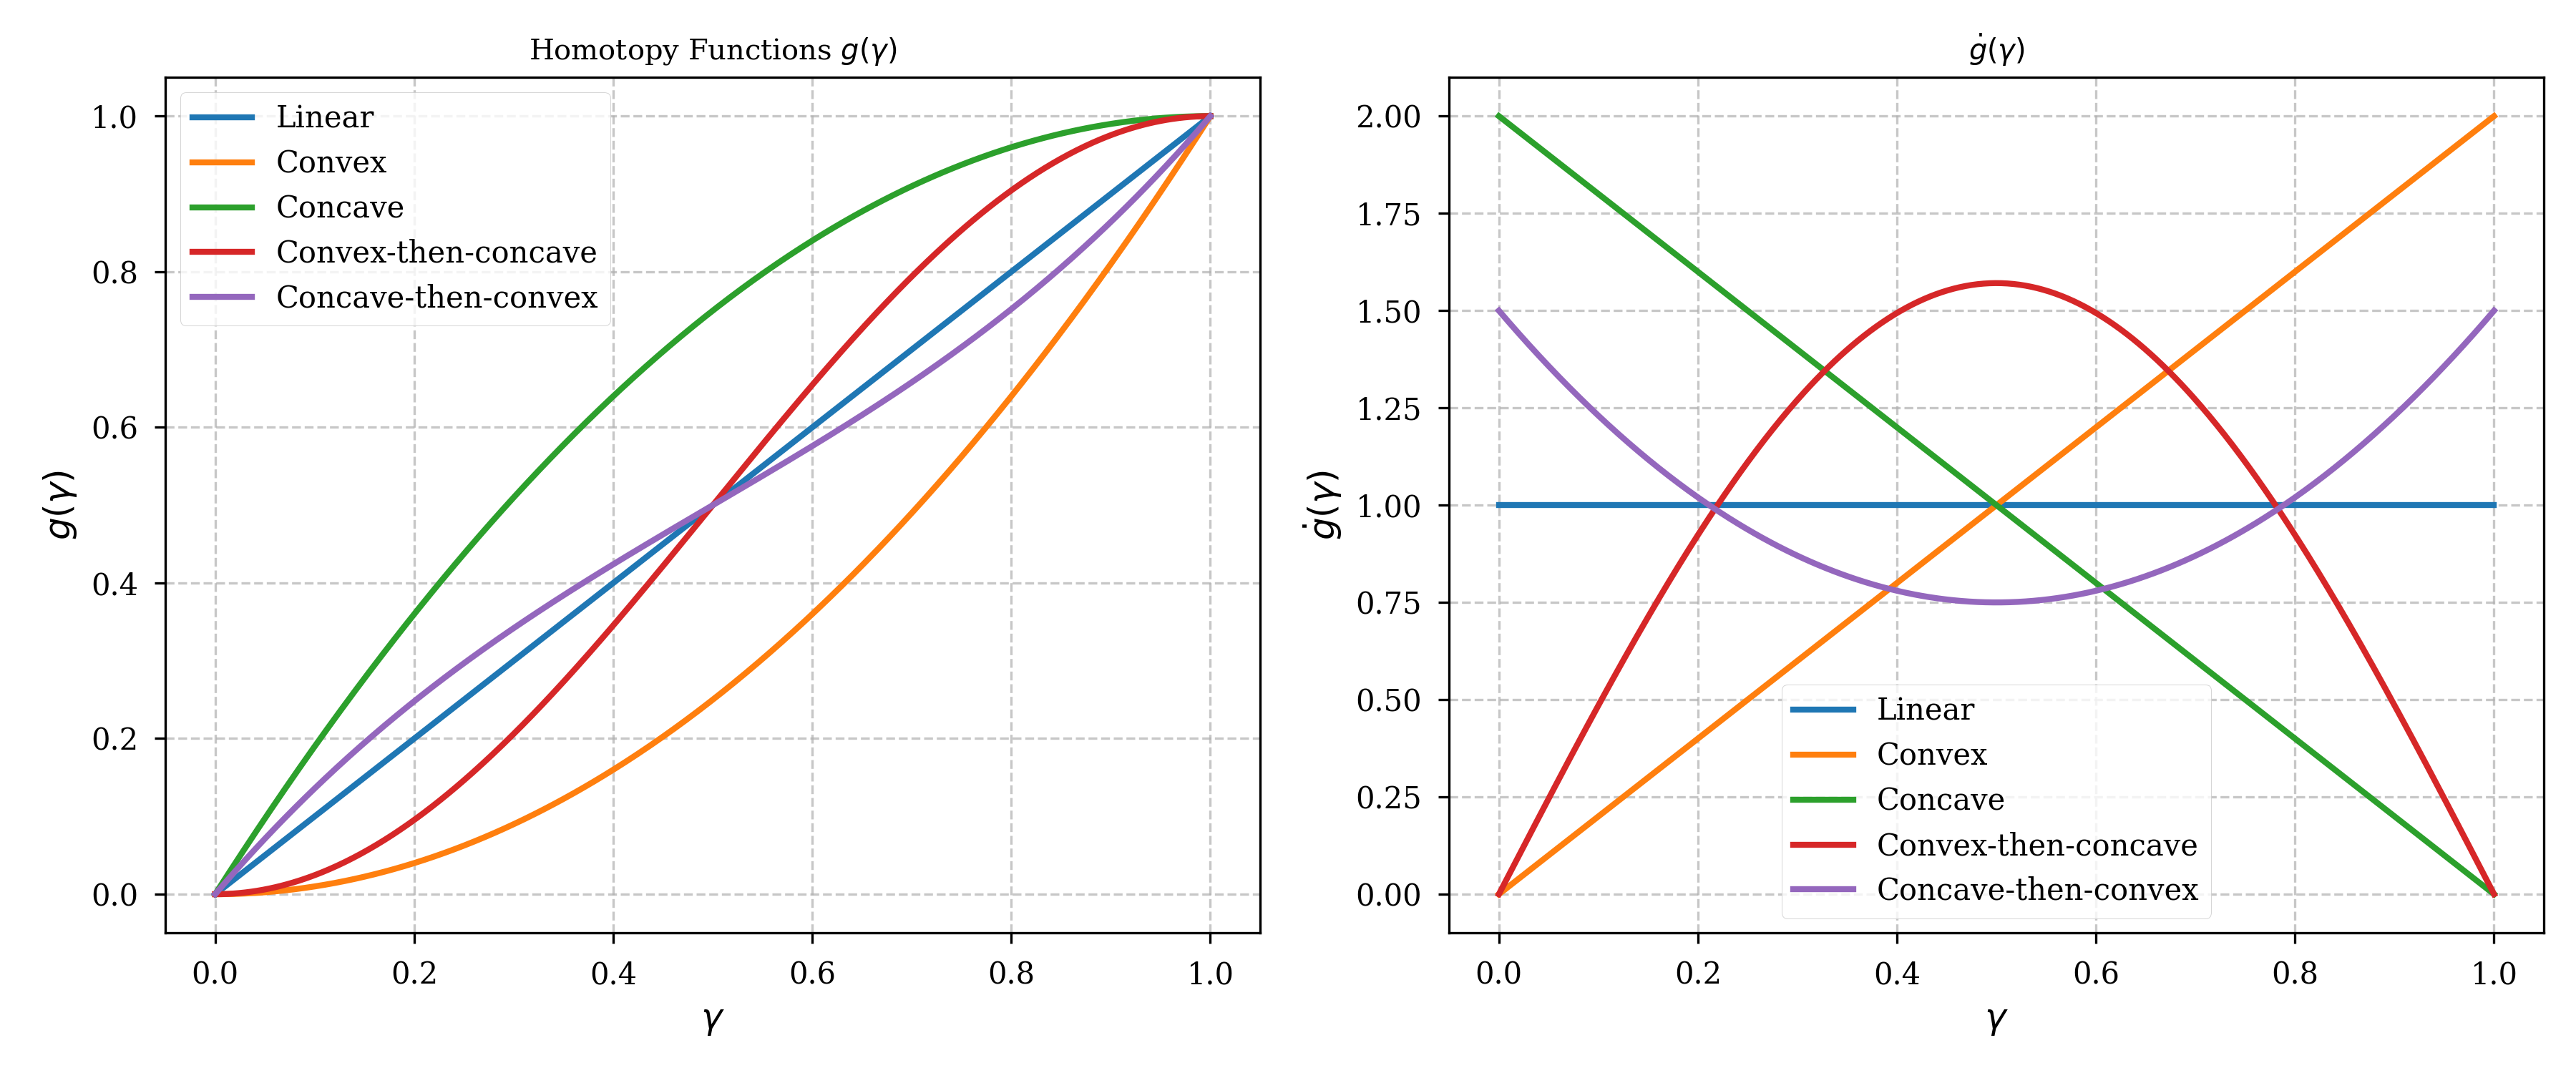
\includegraphics[width=0.95\textwidth]{figures/homotopy_function.png} 
    \caption{Comparison of homotopy functions $g(\gamma)$ and their derivatives $\dot{g}(\gamma)$.}
    \label{fig:function_plots}
\end{Figure}

The experimental results are shown in \Fig{fig:homotopy_results}.

\begin{Figure}[ht]
	\centering
	\begin{SubFigure}{0.48\textwidth}
		\centering
		
\includegraphics[width=\textwidth]{figures/Experiment3.2/rmse.png}
		\caption{RMSE vs. $g(\gamma)$}
		\label{fig:homotopy_rmse}
	\end{SubFigure}
	\hfill
	\begin{SubFigure}{0.48\textwidth}
		\centering
		
\includegraphics[width=\textwidth]{figures/Experiment3.2/rel_frob.png}
		\caption{RFE vs. $g(\gamma)$}
		\label{fig:homotopy_frob}
	\end{SubFigure}
	
	\vspace{1em}
	\begin{SubFigure}{0.48\textwidth}
		\centering
		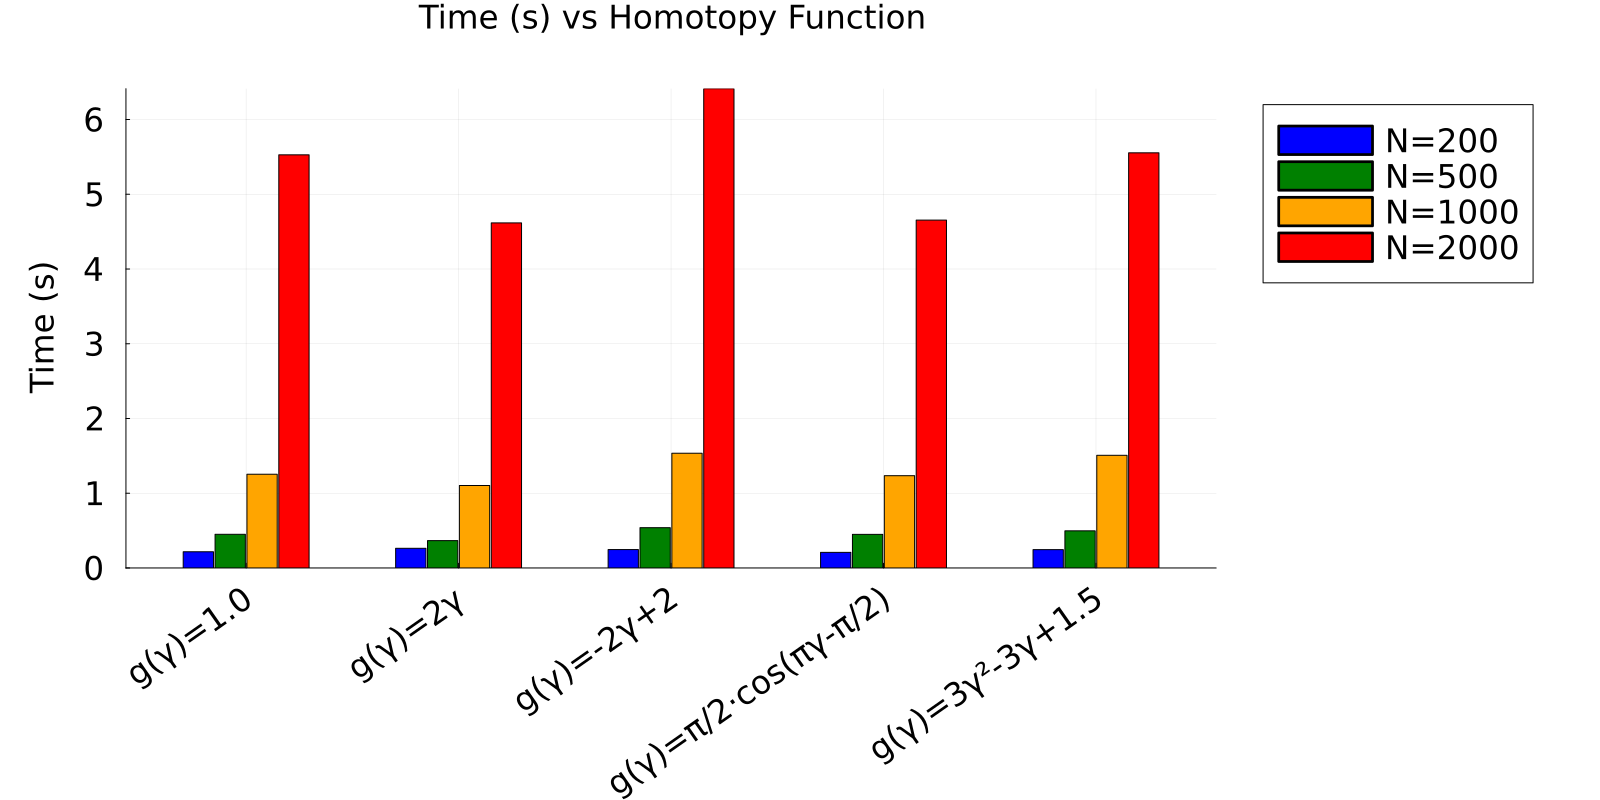
\includegraphics[width=\textwidth]{figures/Experiment3.2/time.png}
		\caption{Computation time vs. $g(\gamma)$}
		\label{fig:homotopy_time}
	\end{SubFigure}
	
	\caption{Accuracy and efficiency vs. $g(\gamma)$.}
	\label{fig:homotopy_results}
\end{Figure}

The bar charts for RMSE and RFE show that, under the same particle configuration, the mean and covariance estimation accuracy is almost identical for all five functions. This indicates that the absolute accuracy of the filter is largely insensitive to the specific shape of the homotopy path.

However, the computation-time plot clearly shows that different homotopy functions lead to noticeable differences in computational cost. In particular, the execution time is substantially reduced when the convex function ($\dot{g}(\gamma)=2\gamma$) or the convex-then-concave function ($\dot{g}(\gamma) = \frac{\pi}{2}\cos(\pi\gamma - \frac{\pi}{2})$) is used. In contrast, the execution time increases significantly for the concave and concave-then-convex functions.

The root cause of these timing differences is that the derivative $\dot{g}(\gamma)$ directly controls the initial stiffness of the ODE. As shown in the previous derivation, during the initial stage of the virtual-time evolution ($\gamma \to 0$), the particle set is still located in the prior region, which is far from the high-probability region of the likelihood and therefore produces a stiff ODE system. If a concave homotopy is used, for example with $\dot{g}(0) = 2$, the stiffness becomes even stronger. By contrast, when a convex or convex-then-concave homotopy is used, with $\dot{g}(0) = 0$, the derivative is initially very small. This small numerical multiplier alleviates the stiffness caused by the large initial distance between the particles and the likelihood region.

Therefore, in practical applications of NFF, a convex or convex-then-concave homotopy function should be preferred. This choice preserves the original estimation accuracy while mitigating the initial stiffness of the ODE, thereby significantly improving computational efficiency.
\clearpage

\subsection{Influence of the Regularization Parameter}
\label{subsec:regularization_parameter}

In the theoretical derivation of NFF, a small regularization parameter $d_{\min}^2$ is introduced to avoid numerical problems when the inter-particle distance approaches zero. To investigate the effect of this parameter, four values of $d_{\min}^2$ with different orders of magnitude ($10^{-24}, 10^{-16}, 10^{-8}, 10^{-3}$) are compared. The results are shown in \Fig{fig:regularization_results}.

\begin{Figure}[ht]
	\centering
	\begin{SubFigure}{0.48\textwidth}
		\centering
		
\includegraphics[width=\textwidth]{figures/Experiment3.3/rmse.png}
		\caption{RMSE vs. $d_{\min}^2$.}
		\label{fig:dmin_rmse}
	\end{SubFigure}
	\hfill
	\begin{SubFigure}{0.48\textwidth}
		\centering
		
\includegraphics[width=\textwidth]{figures/Experiment3.3/rel_frob.png}
		\caption{RFE vs. $d_{\min}^2$.}
		\label{fig:dmin_frob}
	\end{SubFigure}
	
	\vspace{1em}
	
	\begin{SubFigure}{0.48\textwidth}
		\centering
		
\includegraphics[width=\textwidth]{figures/Experiment3.3/time.png}
		\caption{Computation time vs. $d_{\min}^2$.}
		\label{fig:dmin_time}
	\end{SubFigure}
	
	\caption{Accuracy and efficiency vs. $d_{\min}^2$.}
	\label{fig:regularization_results}
\end{Figure}

As shown in the results, both RMSE and RFE worsen as $d_{\min}^2$ increases. In addition, the single-step update time of the algorithm increases significantly with larger values of $d_{\min}^2$.
\clearpage

\subsection{Influence of the Penalty Coefficient}
\label{subsec:penalty_coefficient}

In the CVM distance, the coefficient $K$ acts as a first-moment penalty coefficient. It controls the weight assigned to the mean difference between the two distributions in the total optimization objective. To analyze the effect of this parameter, the experiment evaluates several values of $K$ with different magnitudes.

\begin{Figure}[ht]
	\centering
	\begin{SubFigure}{0.48\textwidth}
		\centering
		
\includegraphics[width=\textwidth]{figures/Experiment3.4/rmse.png}
		\caption{RMSE vs. $K$.}
		\label{fig:penalty_rmse}
	\end{SubFigure}
	\hfill
	\begin{SubFigure}{0.48\textwidth}
		\centering
		
\includegraphics[width=\textwidth]{figures/Experiment3.4/rel_frob.png}
		\caption{RFE vs. $K$.}
		\label{fig:penalty_frob}
	\end{SubFigure}
	
	\caption{RMSE and RFE vs. $K$.}
	\label{fig:penalty_K_results}
\end{Figure}

The results(\Fig{fig:penalty_K_results}) show that as the penalty coefficient $K$ increases, the covariance estimation accuracy of NFF gradually deteriorates. However, once $K$ reaches a sufficiently large value (e.g., $K \ge 100$), the mean estimation error decreases and remains at a highly accurate level.
\clearpage

\section{Limitations in Handling Multimodal Distributions}
\label{sec:multimodal_limitations}

The analysis is carried out in a 10-dimensional state space. The prior distribution is fixed as a standard normal distribution $\Gaussian(\vzero, \mI_{10})$. The likelihood is defined as a bimodal Gaussian mixture with two equally weighted components. The covariance matrices of both modes are fixed at $0.3\mI_{10}$, and their means are located at two distinct points in space:
$\vmu_1 = [5, 5, \dots, 5]^{\top}$ and $\vmu_2 = [-5, -5, \dots, -5]^{\top}$.

\begin{table}[ht]
	\footnotesize
	\setlength{\tabcolsep}{3pt}
	
	\begin{tabularx}{\textwidth}{|X|c|c|c|c|c|c|}
		\hline
		\textbf{Filter} & \textbf{M1 RMSE} & \textbf{M1 RelFrob} & \textbf{M2 RMSE} & \textbf{M2 RelFrob} & \textbf{M1 Count} & \textbf{M2 Count} \\ \hline
		\makecell[l]{NFF\\($L=200$)} & 0.9402 & 0.4778 & N/A & N/A & 200 & 0 \\ \hline
		\makecell[l]{NFF Cov\\($L=200$)} & N/A & N/A & 1.1158 & 0.8741 & 0 & 200 \\ \hline
		\makecell[l]{NFF\\($L=500$)} & N/A & N/A & 1.1046 & 0.4390 & 0 & 500 \\ \hline
		\makecell[l]{NFF Cov\\($L=500$)} & 1.0810 & 0.8291 & N/A & N/A & 500 & 0 \\ \hline
		\makecell[l]{NFF\\($L=1000$)} & 0.9945 & 1.6006 & N/A & N/A & 1000 & 0 \\ \hline
		\makecell[l]{NFF Cov\\($L=1000$)} & 1.4922 & 0.9810 & N/A & N/A & 1000 & 0 \\ \hline
		\makecell[l]{NFF\\($L=2000$)} & 0.9429 & 5.7725 & N/A & N/A & 2000 & 0 \\ \hline
		\makecell[l]{NFF Cov\\($L=2000$)} & 1.0327 & 0.9259 & N/A & N/A & 2000 & 0 \\ \hline
		GPF & 2.8736 & 0.9627 & 2.8069 & 0.9930 & 5002 & 4998 \\ \hline
		PF (avg. 30 runs) & 2.5238 & 1.3845 & 2.5078 & 1.5309 & 149970 & 150030 \\ \hline
	\end{tabularx}
	\caption{Bimodal tracking results: NFF vs. GPF and PF.}
	\label{tab:multimodal_results}
\end{table}

After the update step of NFF, a hyperplane defined by $\sum \vx_i = 0$ is used as a classification boundary to count the particle distribution across the two modes. Particles whose coordinate sum is greater than zero are classified as having moved toward the first mode ($\vmu_1$), whereas particles whose coordinate sum is less than zero are classified as having moved toward the second mode ($\vmu_2$).

In the 10-dimensional bimodal fusion experiment, the particle set of NFF consistently flows as a whole toward only one of the two likelihood modes after the update step is completed. No particles are assigned to the other symmetric mode. This phenomenon is clearly evident from the particle counts recorded in \Tab{tab:multimodal_results}.
\clearpage